\documentclass{../../note}

\usepackage{amsthm}
\usepackage{pgfplots}
\pgfplotsset{compat=1.18}
\newtheorem{example}{Example}

\title{数据结构 01}
\author{isomo}

\begin{document}

\maketitle

\section{绪论}

\subsection{引言}
数据结构是计算机科学中的一门基础课程,它研究数据的组织方式及其操作,对于程序设计、算法设计和计算机系统设计都有着重要的影响。本章将介绍数据结构的基本概念,包括数据、数据元素、数据结构、数据类型、抽象数据类型等,同时也会讨论算法及其分析方法。

\subsection{数据及相关概念}

\subsubsection{数据的概念}
\begin{itemize}
  \item \textbf{数据}(Data):是对客观事物的符号表示,在计算机科学中,是指所有能输入到计算机中并被计算机程序处理的符号的总称。
  \item 数据是计算机程序加工的原料,是信息的载体。
  \item 数据可以是数值型(如1, 2, 3.14等)、文本型(如"Hello")、图形型、音频型等多种形式。
\end{itemize}

\begin{example}
  学生信息系统中的学生姓名、学号、成绩等都是数据。
  天气预报系统中的温度、湿度、气压等也是数据。
\end{example}

\subsubsection{数据元素的概念}
\begin{itemize}
  \item \textbf{数据元素}(Data Element):是数据的基本单位,通常作为一个整体进行考虑。
  \item 也称为记录(Record)、节点(Node)或实体(Entity)。
  \item 一个数据元素可由若干个数据项(Data Item)组成。
\end{itemize}

\begin{example}
  在学生信息系统中,每个学生的完整信息(包括姓名、学号、成绩等)构成一个数据元素。
  在图书管理系统中,每本书的信息(包括书名、作者、ISBN等)是一个数据元素。
\end{example}

\subsubsection{数据项的概念}
\begin{itemize}
  \item \textbf{数据项}(Data Item):是数据的最小单位,是不可分割的基本单位。
  \item 数据项是组成数据元素的基本单位。
\end{itemize}

\begin{example}
  学生信息中的姓名是一个数据项,学号是一个数据项,成绩是一个数据项。
\end{example}

\subsection{数据结构}

\subsubsection{数据结构的定义}
\begin{itemize}
  \item \textbf{数据结构}(Data Structure):是相互之间存在一种或多种特定关系的数据元素的集合。
  \item 数据结构包括三个方面:
    \begin{enumerate}
      \item 数据的逻辑结构
      \item 数据的存储结构(物理结构)
      \item 数据的操作
    \end{enumerate}
\end{itemize}

\subsubsection{数据的逻辑结构}
\begin{itemize}
  \item \textbf{逻辑结构}(Logical Structure):指数据元素之间的逻辑关系,与数据的存储无关。
  \item 主要分为以下四类:
    \begin{enumerate}
      \item \textbf{线性结构}:元素之间是一对一的关系。如线性表、栈、队列等。
      \item \textbf{树形结构}:元素之间是一对多的关系。如树、二叉树等。
      \item \textbf{图形结构}:元素之间是多对多的关系。如图、网络等。
      \item \textbf{集合结构}:元素之间除了同属一个集合外,没有其他关系。
    \end{enumerate}
\end{itemize}

\begin{figure}[h]
  \centering
  \begin{tikzpicture}
    \node[draw, rectangle] (a) at (0,0) {逻辑结构};
    \node[draw, rectangle] (b1) at (-3,-1.5) {线性结构};
    \node[draw, rectangle] (b2) at (-1,-1.5) {树形结构};
    \node[draw, rectangle] (b3) at (1,-1.5) {图形结构};
    \node[draw, rectangle] (b4) at (3,-1.5) {集合结构};

    \draw[->] (a) -- (b1);
    \draw[->] (a) -- (b2);
    \draw[->] (a) -- (b3);
    \draw[->] (a) -- (b4);
  \end{tikzpicture}
  \caption{数据的逻辑结构分类}
\end{figure}

\subsubsection{数据的存储结构}
\begin{itemize}
  \item \textbf{存储结构}(Storage Structure):指数据在计算机中的表示(又称物理结构)。
  \item 存储结构是逻辑结构在计算机中的映射,通过存储单元之间的邻接关系来反映数据元素之间的逻辑关系。
  \item 主要分为以下四类:
    \begin{enumerate}
      \item \textbf{顺序存储结构}:使用一组地址连续的存储单元依次存储数据元素。
      \item \textbf{链式存储结构}:使用一组任意的存储单元存储数据元素,每个元素还存储指向相关元素的指针。
      \item \textbf{索引存储结构}:在存储数据的同时,建立附加的索引表,以便快速访问。
      \item \textbf{散列存储结构}:根据数据元素的关键字直接计算其存储地址。
    \end{enumerate}
\end{itemize}

\begin{figure}[h]
  \centering
  \begin{tikzpicture}
    \node[draw, rectangle] (a) at (0,0) {存储结构};
    \node[draw, rectangle] (b1) at (-3,-1.5) {顺序存储};
    \node[draw, rectangle] (b2) at (-1,-1.5) {链式存储};
    \node[draw, rectangle] (b3) at (1,-1.5) {索引存储};
    \node[draw, rectangle] (b4) at (3,-1.5) {散列存储};

    \draw[->] (a) -- (b1);
    \draw[->] (a) -- (b2);
    \draw[->] (a) -- (b3);
    \draw[->] (a) -- (b4);
  \end{tikzpicture}
  \caption{数据的存储结构分类}
\end{figure}

\subsection{数据类型与抽象数据类型}

\subsubsection{数据类型}
\begin{itemize}
  \item \textbf{数据类型}(Data Type):是一组性质相同的值的集合及定义在此集合上的一组操作的总称。
  \item 数据类型可以分为两类:
    \begin{enumerate}
      \item \textbf{原子类型}(基本类型):不可再分的类型,如整数、实数、字符等。
      \item \textbf{结构类型}:由多个类型组合而成,如数组、结构体等。
    \end{enumerate}
  \item 在编程语言中,声明变量时必须指定数据类型,如int、float、char等。
\end{itemize}

\subsubsection{抽象数据类型}
\begin{itemize}
  \item \textbf{抽象数据类型}(Abstract Data Type, ADT):是一个数学模型及定义在该模型上的一组操作,它与存储结构的实现无关。
  \item ADT由两部分组成:
    \begin{enumerate}
      \item 数据对象的抽象描述
      \item 对数据对象的操作的抽象描述
    \end{enumerate}
  \item ADT的表示方法:
    \begin{verbatim}
    ADT 抽象数据类型名 {
        数据对象: <数据对象的定义>
        数据关系: <数据关系的定义>
        基本操作: <基本操作的定义>
    }
    \end{verbatim}
\end{itemize}

\begin{example}[抽象数据类型示例]
  以"线性表"为例,其ADT可表示为:
\begin{verbatim}
ADT List {
    数据对象:
        D = {a_i | a_i ∈ ElemSet, i = 1, 2, ..., n, n ≥ 0}
    数据关系:
        R = {<a_i, a_{i+1}> | a_i, a_{i+1} ∈ D, i = 1, 2, ..., n-1}
    基本操作:
        InitList(&L)   // 初始化线性表
        Length(L)      // 求表长
        GetElem(L, i, &e)  // 获取第i个元素
        LocateElem(L, e)   // 查找元素e的位置
        Insert(&L, i, e)   // 在位置i插入元素e
        Delete(&L, i, &e)  // 删除位置i的元素
        ...
}
\end{verbatim}
\end{example}

\subsection{算法及其分析}

\subsubsection{算法的概念}
\begin{itemize}
  \item \textbf{算法}(Algorithm):是解决特定问题的一系列操作的有限序列。
  \item 算法的五个基本特性:
    \begin{enumerate}
      \item \textbf{有穷性}:算法必须在有限步骤内结束。
      \item \textbf{确定性}:算法的每一步骤必须有确定的含义,不能有歧义。
      \item \textbf{可行性}:算法的每一步操作都必须是可行的,即能够通过已经实现的基本操作执行有限次来实现。
      \item \textbf{输入}:算法可以有零个或多个输入。
      \item \textbf{输出}:算法必须有一个或多个输出。
    \end{enumerate}
\end{itemize}

\subsubsection{算法的描述}
算法可以通过多种方式描述:
\begin{enumerate}
  \item \textbf{自然语言}:使用日常语言描述算法步骤。
  \item \textbf{流程图}:使用图形符号表示算法的流程。
  \item \textbf{伪代码}:介于自然语言和程序设计语言之间的描述方式。
  \item \textbf{程序设计语言}:如C、Java等。
\end{enumerate}

\begin{example}[简单算法示例:顺序查找]
  伪代码描述:
\begin{verbatim}
Algorithm SequentialSearch(A[0...n-1], key):
    i = 0
    while i < n and A[i] != key do
        i = i + 1
    if i < n then
        return i  // 找到元素,返回位置
    else
        return -1 // 未找到元素,返回-1
\end{verbatim}
\end{example}

\subsubsection{算法的分析}
算法分析的两个主要方面:
\begin{enumerate}
  \item \textbf{正确性分析}:证明算法是否能正确地解决问题。
  \item \textbf{效率分析}:评估算法的时间复杂度和空间复杂度。
    \begin{itemize}
      \item \textbf{时间复杂度}:算法执行所需的时间。
      \item \textbf{空间复杂度}:算法执行所需的存储空间。
    \end{itemize}
\end{enumerate}

\paragraph{渐进符号}
用于表示算法时间复杂度的常用符号:
\begin{itemize}
  \item \textbf{O(大O)}:表示上界,如O(n²)表示算法的执行时间不超过n²的常数倍。
  \item \textbf{Ω(大Omega)}:表示下界,如Ω(n)表示算法的执行时间至少是n的常数倍。
  \item \textbf{Θ(大Theta)}:表示确界,如Θ(n)表示算法的执行时间恰好是n的常数倍。
\end{itemize}

\paragraph{常见的时间复杂度}
按照效率从高到低排序:
\begin{itemize}
  \item O(1):常数时间,与输入规模无关。
  \item O(log n):对数时间,如二分查找。
  \item O(n):线性时间,如顺序查找。
  \item O(n log n):线性对数时间,如归并排序、快速排序。
  \item O(n²):平方时间,如冒泡排序、插入排序。
  \item O(n³):立方时间,如某些矩阵运算。
  \item O($2^n$):指数时间,如穷举法。
\end{itemize}

\begin{figure}[h]
  \centering
  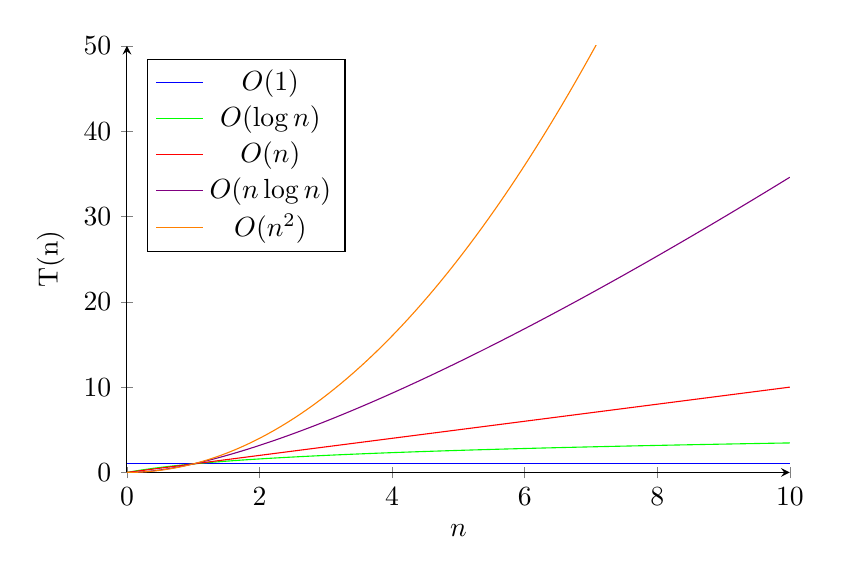
\begin{tikzpicture}
    \begin{axis}[
        domain=0:10,
        samples=100,
        axis lines=left,
        xlabel={$n$},
        ylabel={T(n)},
        legend pos=north west,
        width=10cm,
        height=7cm,
        ymax=50,
      ]
      \addplot[color=blue] {1};
      \addlegendentry{$O(1)$}

      \addplot[color=green] {ln(x+1)/ln(2)};
      \addlegendentry{$O(\log n)$}

      \addplot[color=red] {x};
      \addlegendentry{$O(n)$}

      \addplot[color=violet] {x*ln(x+1)/ln(2)};
      \addlegendentry{$O(n \log n)$}

      \addplot[color=orange] {x^2};
      \addlegendentry{$O(n^2)$}

    \end{axis}
  \end{tikzpicture}
  \caption{常见时间复杂度函数的增长趋势}
\end{figure}

\paragraph{算法效率分析实例}
\begin{example}[顺序查找算法的时间复杂度分析]
  顺序查找算法的最坏情况:要查找的元素在数组的最后或不存在,需要比较n次,时间复杂度为O(n)。
  最好情况:要查找的元素在数组的第一个位置,只需比较1次,时间复杂度为O(1)。
  平均情况:假设查找任意位置的概率相等,则平均需要比较(n+1)/2次,时间复杂度仍为O(n)。
\end{example}

\subsection{数据结构的应用}

数据结构在计算机科学和实际应用中具有广泛的应用:

\begin{itemize}
  \item \textbf{数据库系统}:利用各种数据结构组织和存储数据,实现高效的数据管理。
  \item \textbf{操作系统}:利用队列管理进程,利用树结构管理文件系统等。
  \item \textbf{编译器}:利用栈实现表达式求值,利用树结构表示语法分析等。
  \item \textbf{搜索引擎}:利用倒排索引等数据结构实现高效的信息检索。
  \item \textbf{图形处理}:利用图和树等结构描述图像和几何对象的关系。
  \item \textbf{人工智能}:利用各种数据结构表示知识和实现搜索算法。
\end{itemize}

\subsection{本章小结}
本章介绍了数据结构的基本概念,包括数据、数据元素、数据项、数据的逻辑结构和存储结构、数据类型和抽象数据类型等。同时,也讨论了算法的概念、算法的描述方法以及算法分析的基本方法,特别是时间复杂度和空间复杂度的概念和分析方法。这些基础知识是学习后续各种具体数据结构和算法的必要前提。

\section{线性表}

\subsection{线性表的基本概念}

\subsubsection{线性表的定义}
\begin{itemize}
  \item \textbf{线性表}(Linear List)是具有相同数据类型的n个数据元素的有限序列。
  \item 其中,n为表长度,当n=0时称为空表。
  \item 线性表中元素的位序(Position)是从1开始的。
  \item 若用$L$表示线性表,则记为:$L = (a_1, a_2, \ldots, a_n)$
  \item 线性表中元素的特点:
    \begin{enumerate}
      \item 除第一个元素外,每个元素有且仅有一个直接前驱。
      \item 除最后一个元素外,每个元素有且仅有一个直接后继。
    \end{enumerate}
\end{itemize}

\begin{figure}[h]
  \centering
  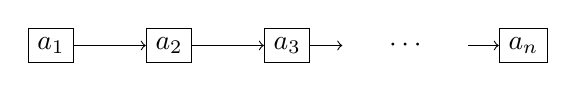
\begin{tikzpicture}
    \node[draw, rectangle] (a1) at (0,0) {$a_1$};
    \node[draw, rectangle] (a2) at (1.5,0) {$a_2$};
    \node[draw, rectangle] (a3) at (3,0) {$a_3$};
    \node at (4.5,0) {$\cdots$};
    \node[draw, rectangle] (an) at (6,0) {$a_n$};

    \draw[->] (a1) -- (a2);
    \draw[->] (a2) -- (a3);
    \draw[->] (a3) -- (3.7,0);
    \draw[->] (5.3,0) -- (an);
  \end{tikzpicture}
  \caption{线性表的逻辑结构}
\end{figure}

\subsubsection{线性表的抽象数据类型描述}

线性表的抽象数据类型(ADT)描述如下:

\begin{verbatim}
ADT LinearList {
    数据对象:
        D = {a_i | a_i ∈ ElementSet, i = 1, 2, ..., n, n ≥ 0}
    数据关系:
        R = {<a_i, a_{i+1}> | a_i, a_{i+1} ∈ D, i = 1, 2, ..., n-1}
    基本操作:
        InitList(&L)            // 初始化线性表
        DestroyList(&L)         // 销毁线性表
        ClearList(&L)           // 清空线性表
        ListEmpty(L)            // 判断线性表是否为空
        ListLength(L)           // 获取线性表长度
        GetElem(L, i, &e)       // 获取第i个元素
        LocateElem(L, e, compare)  // 查找元素e
        PriorElem(L, cur_e, &pre_e)  // 获取元素cur_e的前驱
        NextElem(L, cur_e, &next_e)  // 获取元素cur_e的后继
        ListInsert(&L, i, e)    // 在第i个位置插入元素e
        ListDelete(&L, i, &e)   // 删除第i个元素
        ListTraverse(L, visit)  // 遍历线性表
}
\end{verbatim}

\subsection{线性表的顺序表示}

\subsubsection{顺序表的定义}
\begin{itemize}
  \item \textbf{顺序表}是用一组地址连续的存储单元依次存储线性表中的数据元素,使得逻辑上相邻的两个元素在物理位置上也相邻。
  \item 顺序表是线性表的顺序存储结构。
  \item 优点:
    \begin{enumerate}
      \item 随机访问特性:可以在$O(1)$时间内访问任意位置的元素。
      \item 无须为表中元素之间的逻辑关系增加额外的存储空间。
    \end{enumerate}
  \item 缺点:
    \begin{enumerate}
      \item 插入和删除操作需要移动大量元素,效率较低。
      \item 存储空间需要预先分配,可能会出现内存浪费或溢出的情况。
    \end{enumerate}
\end{itemize}

\subsubsection{顺序表的存储结构}

\paragraph{静态分配}
在C语言中,可以用数组来实现顺序表的静态分配:

\begin{verbatim}
#define MAXSIZE 100  // 顺序表的最大长度

typedef struct {
    ElemType data[MAXSIZE];  // 数组,存储数据元素
    int length;             // 当前长度
} SqList;
\end{verbatim}

\paragraph{动态分配}
在C语言中,可以用指针和动态内存分配来实现顺序表的动态分配:

\begin{verbatim}
typedef struct {
    ElemType *data;  // 指向动态分配数组的指针
    int maxSize;     // 顺序表的最大容量
    int length;      // 顺序表的当前长度
} SqList;
\end{verbatim}

\begin{figure}[h]
  \centering
  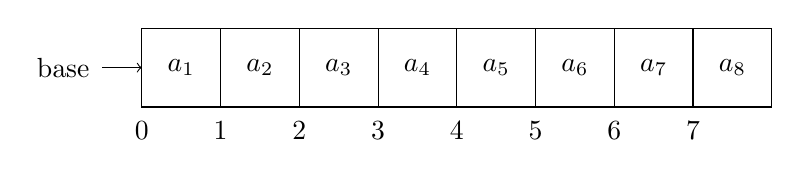
\begin{tikzpicture}
    \draw (0,0) rectangle (8,1);
    \foreach \x in {1,2,...,7}
    \draw (\x,0) -- (\x,1);
    \node at (0.5,0.5) {$a_1$};
    \node at (1.5,0.5) {$a_2$};
    \node at (2.5,0.5) {$a_3$};
    \node at (3.5,0.5) {$a_4$};
    \node at (4.5,0.5) {$a_5$};
    \node at (5.5,0.5) {$a_6$};
    \node at (6.5,0.5) {$a_7$};
    \node at (7.5,0.5) {$a_8$};
    \node at (0,-0.3) {0};
    \node at (1,-0.3) {1};
    \node at (2,-0.3) {2};
    \node at (3,-0.3) {3};
    \node at (4,-0.3) {4};
    \node at (5,-0.3) {5};
    \node at (6,-0.3) {6};
    \node at (7,-0.3) {7};

    \draw[->] (-0.5,0.5) -- (0,0.5);
    \node at (-1,0.5) {base};
  \end{tikzpicture}
  \caption{顺序表的存储结构}
\end{figure}

\subsubsection{顺序表的基本运算}

\paragraph{顺序表的初始化}
\begin{verbatim}
Status InitList_Sq(SqList &L) {
    // 为顺序表分配一个大小为MAXSIZE的数组空间
    L.data = new ElemType[MAXSIZE];
    if (!L.data) return ERROR;  // 存储分配失败
    L.length = 0;               // 空表长度为0
    L.maxSize = MAXSIZE;        // 最大长度为MAXSIZE
    return OK;
}
\end{verbatim}

\paragraph{顺序表的取值}
根据位置$i$获取相应位置数据元素$e$的值,时间复杂度为$O(1)$。

\begin{verbatim}
Status GetElem_Sq(SqList L, int i, ElemType &e) {
    if (i < 1 || i > L.length) return ERROR;  // i值不合法
    e = L.data[i-1];                          // 第i-1个单元存储第i个元素
    return OK;
}
\end{verbatim}

\paragraph{顺序表的查找}
在顺序表L中查找值为e的元素,若找到,则返回其位序;否则,返回0。

\begin{verbatim}
int LocateElem_Sq(SqList L, ElemType e) {
    for (int i = 0; i < L.length; i++)
        if (L.data[i] == e) return i+1;  // 返回位序
    return 0;  // 查找失败,返回0
}
\end{verbatim}

顺序查找的平均时间复杂度为$O(n)$。

\paragraph{顺序表的插入}
在顺序表L的第i个位置插入新元素e。

\begin{verbatim}
Status ListInsert_Sq(SqList &L, int i, ElemType e) {
    if (i < 1 || i > L.length + 1) return ERROR;  // i值不合法
    if (L.length >= L.maxSize) return ERROR;      // 当前存储空间已满

    // 将第i个位置后的元素向后移动
    for (int j = L.length; j >= i; j--)
        L.data[j] = L.data[j-1];

    L.data[i-1] = e;  // 插入新元素
    L.length++;       // 表长增加1
    return OK;
}
\end{verbatim}

\begin{figure}[h]
  \centering
  \begin{tikzpicture}
    % 原始顺序表
    \draw (0,2) rectangle (6,3);
    \foreach \x in {1,2,3,4,5}
    \draw (\x,2) -- (\x,3);
    \node at (0.5,2.5) {$a_1$};
    \node at (1.5,2.5) {$a_2$};
    \node at (2.5,2.5) {$a_3$};
    \node at (3.5,2.5) {$a_4$};
    \node at (4.5,2.5) {$a_5$};
    \node at (5.5,2.5) {$a_6$};

    % 插入后
    \draw (0,0) rectangle (7,1);
    \foreach \x in {1,2,3,4,5,6}
    \draw (\x,0) -- (\x,1);
    \node at (0.5,0.5) {$a_1$};
    \node at (1.5,0.5) {$a_2$};
    \node at (2.5,0.5) {$e$};
    \node at (3.5,0.5) {$a_3$};
    \node at (4.5,0.5) {$a_4$};
    \node at (5.5,0.5) {$a_5$};
    \node at (6.5,0.5) {$a_6$};

    % 箭头和说明
    \draw[->] (2.5,1.5) -- (2.5,1);
    \node at (3.3,1.5) {插入到第3个位置};
  \end{tikzpicture}
  \caption{顺序表的插入操作示意图}
\end{figure}

顺序表插入操作的时间复杂度分析:
\begin{itemize}
  \item 最好情况:插入到表尾,无需移动元素,时间复杂度为$O(1)$。
  \item 最坏情况:插入到表头,需要移动所有元素,时间复杂度为$O(n)$。
  \item 平均情况:假设插入位置均匀分布,平均需要移动$n/2$个元素,时间复杂度为$O(n)$。
\end{itemize}

\paragraph{顺序表的删除}
删除顺序表L中第i个元素,并用e返回其值。

\begin{verbatim}
Status ListDelete_Sq(SqList &L, int i, ElemType &e) {
    if (i < 1 || i > L.length) return ERROR;  // i值不合法

    e = L.data[i-1];  // 保存被删除元素

    // 将第i个位置后的元素向前移动
    for (int j = i; j < L.length; j++)
        L.data[j-1] = L.data[j];

    L.length--;       // 表长减少1
    return OK;
}
\end{verbatim}

\begin{figure}[h]
  \centering
  \begin{tikzpicture}
    % 原始顺序表
    \draw (0,2) rectangle (6,3);
    \foreach \x in {1,2,3,4,5}
    \draw (\x,2) -- (\x,3);
    \node at (0.5,2.5) {$a_1$};
    \node at (1.5,2.5) {$a_2$};
    \node at (2.5,2.5) {$a_3$};
    \node at (3.5,2.5) {$a_4$};
    \node at (4.5,2.5) {$a_5$};
    \node at (5.5,2.5) {$a_6$};

    % 删除后
    \draw (0,0) rectangle (5,1);
    \foreach \x in {1,2,3,4}
    \draw (\x,0) -- (\x,1);
    \node at (0.5,0.5) {$a_1$};
    \node at (1.5,0.5) {$a_2$};
    \node at (2.5,0.5) {$a_4$};
    \node at (3.5,0.5) {$a_5$};
    \node at (4.5,0.5) {$a_6$};

    % 箭头和说明
    \draw[->] (2.5,2) -- (2.5,1.5);
    \node at (3.3,1.5) {删除第3个元素};
  \end{tikzpicture}
  \caption{顺序表的删除操作示意图}
\end{figure}

顺序表删除操作的时间复杂度分析:
\begin{itemize}
  \item 最好情况:删除表尾元素,无需移动元素,时间复杂度为$O(1)$。
  \item 最坏情况:删除表头元素,需要移动所有元素,时间复杂度为$O(n)$。
  \item 平均情况:假设删除位置均匀分布,平均需要移动$(n-1)/2$个元素,时间复杂度为$O(n)$。
\end{itemize}

\paragraph{顺序表的排序}
常用的排序算法包括冒泡排序、选择排序、插入排序、希尔排序、快速排序、堆排序、归并排序等。

以冒泡排序为例:
\begin{verbatim}
void BubbleSort(SqList &L) {
    for (int i = 0; i < L.length - 1; i++) {
        bool flag = false;  // 标记本轮是否有交换
        for (int j = 0; j < L.length - 1 - i; j++) {
            if (L.data[j] > L.data[j+1]) {  // 相邻元素比较
                // 交换元素
                ElemType temp = L.data[j];
                L.data[j] = L.data[j+1];
                L.data[j+1] = temp;
                flag = true;  // 本轮有交换
            }
        }
        if (!flag) break;  // 本轮无交换,说明已经有序
    }
}
\end{verbatim}

\subsection{线性表的链式表示}

\subsubsection{链表的基本概念}
\begin{itemize}
  \item \textbf{链表}是线性表的链式存储结构,它使用一组任意的存储单元来存储线性表中的数据元素。
  \item 链表中的每个元素(称为结点)在存储数据的同时,还存储指向下一个结点的指针(或引用)。
  \item 链表不要求逻辑上相邻的元素在物理位置上也相邻。
  \item 优点:
    \begin{enumerate}
      \item 插入和删除操作不需要移动元素,时间复杂度为$O(1)$(不考虑查找时间)。
      \item 充分利用计算机内存空间,不会出现内存浪费。
    \end{enumerate}
  \item 缺点:
    \begin{enumerate}
      \item 不支持随机访问,访问特定位置的元素需要$O(n)$的时间复杂度。
      \item 需要额外的存储空间来存储指针信息。
    \end{enumerate}
\end{itemize}

\subsubsection{单链表}

\paragraph{单链表的节点结构}
在C语言中,单链表的节点结构如下:

\begin{verbatim}
typedef struct LNode {
    ElemType data;         // 数据域
    struct LNode *next;    // 指针域,指向下一个节点
} LNode, *LinkList;        // LinkList为指向LNode的指针类型
\end{verbatim}

\begin{figure}[h]
  \centering
  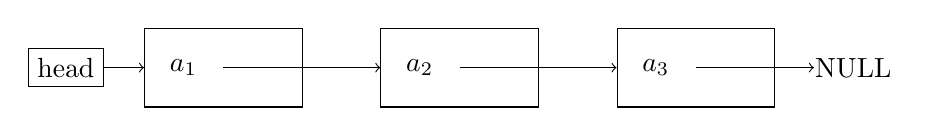
\begin{tikzpicture}
    % 头指针
    \node[draw, rectangle] (head) at (0,0) {head};

    % 节点
    \node[draw, rectangle, minimum width=2cm, minimum height=1cm] (node1) at (2,0) {};
    \node[draw, rectangle, minimum width=2cm, minimum height=1cm] (node2) at (5,0) {};
    \node[draw, rectangle, minimum width=2cm, minimum height=1cm] (node3) at (8,0) {};

    % 节点内部
    \draw (node1.center) -- (node1.east);
    \draw (node2.center) -- (node2.east);
    \draw (node3.center) -- (node3.east);

    \node at (node1.west) [xshift=0.5cm] {$a_1$};
    \node at (node2.west) [xshift=0.5cm] {$a_2$};
    \node at (node3.west) [xshift=0.5cm] {$a_3$};

    % 指针
    \draw[->] (head) -- (node1);
    \draw[->] (node1.east) -- (node2.west);
    \draw[->] (node2.east) -- (node3.west);
    \draw[->] (node3.east) -- (9.5,0);
    \node at (10,0) {NULL};
  \end{tikzpicture}
  \caption{单链表示意图}
\end{figure}

\paragraph{单链表的创建方式}

1. 头插法(逆序建立)
\begin{verbatim}
LinkList CreateList_H() {
    LinkList L = (LinkList)malloc(sizeof(LNode));  // 创建头节点
    L->next = NULL;                                // 初始为空链表

    int n;
    printf("请输入元素个数:");
    scanf("%d", &n);

    for (int i = 0; i < n; i++) {
        LinkList p = (LinkList)malloc(sizeof(LNode));  // 创建新节点
        scanf("%d", &(p->data));                       // 输入元素值
        p->next = L->next;   // 将新节点插入表头
        L->next = p;
    }

    return L;
}
\end{verbatim}

\begin{figure}[h]
  \centering
  \begin{tikzpicture}
    % 头节点
    \node[draw, circle] (head) at (0,0) {L};

    % 初始状态
    \draw[->] (head) -- (1,0);
    \node at (1.5,0) {NULL};

    % 加入第一个节点
    \node[draw, rectangle, minimum width=2cm, minimum height=1cm] (node1) at (4,3) {};
    \draw (node1.center) -- (node1.east);
    \node at (4,3.5) {新节点p};
    \node at (node1.west) [xshift=0.5cm] {$a_1$};
    \draw[->] (node1.east) -- (5.5,3);
    \node at (6,3) {NULL};

    \draw[->, dashed] (node1.east) -- (1,0.3);
    \draw[->, dashed] (head) -- (3,3);

    % 加入第二个节点
    \node[draw, rectangle, minimum width=2cm, minimum height=1cm] (node2) at (4,1.5) {};
    \draw (node2.center) -- (node2.east);
    \node at (4,2) {新节点p};
    \node at (node2.west) [xshift=0.5cm] {$a_2$};

    \draw[->, dashed] (node2.east) -- (node1.west);
    \draw[->, dashed] (head) -- (3,1.5);

    % 最终结果
    \node[draw, rectangle, minimum width=2cm, minimum height=1cm] (result1) at (4,0) {};
    \node[draw, rectangle, minimum width=2cm, minimum height=1cm] (result2) at (7,0) {};

    \draw (result1.center) -- (result1.east);
    \draw (result2.center) -- (result2.east);

    \node at (result1.west) [xshift=0.5cm] {$a_2$};
    \node at (result2.west) [xshift=0.5cm] {$a_1$};

    \draw[->] (head) -- (result1);
    \draw[->] (result1.east) -- (result2.west);
    \draw[->] (result2.east) -- (8.5,0);
    \node at (9,0) {NULL};
  \end{tikzpicture}
  \caption{单链表头插法示意图}
\end{figure}

2. 尾插法(正序建立)
\begin{verbatim}
LinkList CreateList_T() {
    LinkList L = (LinkList)malloc(sizeof(LNode));  // 创建头节点
    L->next = NULL;                                // 初始为空链表
    LNode *r = L;                                  // r指向尾节点,初始时指向头节点

    int n;
    printf("请输入元素个数:");
    scanf("%d", &n);

    for (int i = 0; i < n; i++) {
        LinkList p = (LinkList)malloc(sizeof(LNode));  // 创建新节点
        scanf("%d", &(p->data));                       // 输入元素值
        p->next = NULL;      // 新节点暂时是尾节点
        r->next = p;         // 将新节点插入到尾节点之后
        r = p;               // r指向新的尾节点
    }

    return L;
}
\end{verbatim}

\paragraph{单链表的基本操作}

1. 获取链表长度
\begin{verbatim}
int GetLength(LinkList L) {
    int length = 0;
    LinkList p = L->next;  // 从第一个节点开始

    while (p) {
        length++;
        p = p->next;
    }

    return length;
}
\end{verbatim}

2. 按位置查找节点
\begin{verbatim}
LNode* GetElem(LinkList L, int i) {
    if (i < 0) return NULL;  // i不合法

    int j = 0;
    LinkList p = L;  // 从头节点开始,j=0表示头节点

    while (p && j < i) {
        p = p->next;
        j++;
    }

    return p;  // 返回第i个节点
}
\end{verbatim}

3. 按值查找节点
\begin{verbatim}
LNode* LocateElem(LinkList L, ElemType e) {
    LinkList p = L->next;  // 从第一个节点开始

    while (p && p->data != e)
        p = p->next;

    return p;  // 找到返回节点指针,否则返回NULL
}
\end{verbatim}

4. 插入节点
在第i个位置插入值为e的新节点。

\begin{verbatim}
Status ListInsert(LinkList &L, int i, ElemType e) {
    LinkList p = GetElem(L, i-1);  // 查找第i-1个节点
    if (!p) return ERROR;          // i-1位置不存在

    LinkList s = (LinkList)malloc(sizeof(LNode));  // 创建新节点
    s->data = e;                                  // 赋值

    s->next = p->next;  // 新节点指向原第i个节点
    p->next = s;        // 第i-1个节点指向新节点

    return OK;
}
\end{verbatim}

\begin{figure}[h]
  \centering
  \begin{tikzpicture}
    % 原始链表
    \node[draw, rectangle, minimum width=2cm, minimum height=1cm] (node1) at (0,2) {};
    \node[draw, rectangle, minimum width=2cm, minimum height=1cm] (node2) at (3,2) {};
    \node[draw, rectangle, minimum width=2cm, minimum height=1cm] (node3) at (6,2) {};

    \draw (node1.center) -- (node1.east);
    \draw (node2.center) -- (node2.east);
    \draw (node3.center) -- (node3.east);

    \node at (node1.west) [xshift=0.5cm] {$a_1$};
    \node at (node2.west) [xshift=0.5cm] {$a_2$};
    \node at (node3.west) [xshift=0.5cm] {$a_3$};

    \draw[->] (node1.east) -- (node2.west);
    \draw[->] (node2.east) -- (node3.west);
    \draw[->] (node3.east) -- (7.5,2);
    \node at (8,2) {NULL};

    % 新节点
    \node[draw, rectangle, minimum width=2cm, minimum height=1cm] (newnode) at (3,0) {};
    \draw (newnode.center) -- (newnode.east);
    \node at (newnode.west) [xshift=0.5cm] {$e$};
    \node at (3,-0.5) {新节点};

    % 插入后的链表
    \draw[->, dashed] (newnode.east) -- (node3.west);
    \draw[->, dashed] (node2.east) -- (newnode.west);
  \end{tikzpicture}
  \caption{单链表的插入操作}
\end{figure}

5. 删除节点
删除第i个节点。

\begin{verbatim}
Status ListDelete(LinkList &L, int i, ElemType &e) {
    LinkList p = GetElem(L, i-1);  // 查找第i-1个节点
    if (!p || !p->next) return ERROR;  // i-1位置不存在或第i个节点不存在

    LinkList q = p->next;    // q指向待删除节点
    e = q->data;            // 保存被删除节点的值

    p->next = q->next;      // 第i-1个节点指向第i+1个节点
    free(q);                // 释放被删除节点的空间

    return OK;
}
\end{verbatim}

\end{document}